\documentclass[11pt]{article}
\usepackage{tikz}
%\usepackage{xfrac}
%\usepackage{hyperref}
%\usepackage[export]{adjustbox}
\def\checkmark{\tikz\fill[scale=0.4](0,.35) -- (.25,0) -- (1,.7) -- (.25,.15) -- cycle;} 
\usepackage{proj} 	% pull in style header
\usepackage{array}
\usepackage{sectsty}

\lhead{ECE540: SoC Design with FPGA's}

%TODO: Put in coverpage from hw1, with tunnel vision image.  

%----------------------------------------------------------------------------------------
%	TITLE SECTION
%----------------------------------------------------------------------------------------


\newcommand{\horrule}[1]{\rule{\linewidth}{#1}} % Create horizontal rule command with 1 argument of height

\title{	
\normalfont \normalsize 
\textsc{\LARGE Portland State University}\\[1.5cm] % Name of your university/college
\textsc{\Large SoC Design With FPGAs}\\[0.5cm] % Major heading such as course name
\textsc{\large ECE540}\\[0.5cm] % Minor heading such as course title
%\textsc{Portland State University} \\ [25pt] % Your university, school and/or department name(s)
\horrule{1.2pt} \\[0.4cm] % Thin top horizontal rule
\huge Tunnel Vision \\ % The assignment title
\horrule{1.2pt} \\[0.5cm] % Thick bottom horizontal rule
}

%----------------------------------------------------------------------------------------
%	AUTHOR SECTION
%----------------------------------------------------------------------------------------


\begin{document}\raggedright
\author{Erik Rhodes \and Bhavana Dhulipala \and Rohan Deshpande \and Nikhil Patil} % Your name
\maketitle % Print the title
\thispagestyle{empty}
\cfoot{\textit{Page \thepage { of} \pageref{LastPage}}}
\lhead{ECE540: SoC Design}
\chead{github.com/rhodeser/tunnel-vision}
\rhead{Tunnel Vision}


\begin{figure}[h]\centering
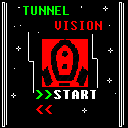
\includegraphics[height=0.65\textwidth]{Images/start.png}
	%\caption{Gameplay Block Diagram}
		\label{start}
	\end{figure}

\tableofcontents
\newpage
%Start of Document

% PUT IN CODE?
% put in design specs - Pictures: Top module, Hardware specifications?

\section{Introduction} 
\textbf{Tunnel Vision} is a racing game that can be played on the \textbf{Xilinx Nexys3 FPGA} board and be displayed on a VGA monitor.

\subsection{Gameplay}
The player tries to avoid hitting the vehicle against the walls or obstacles as it travels down the tunnel. The space in between the walls steadily decreases until the player hits a wall or obstacle. The score is based on the amount of time the vehicle remains ``alive'', and is displayed on the 7-segment display.

\subsection{Controls}
The player can move the vehicle by using the left and right push buttons on the Nexys3. When the game is over, hitting the middle button will reset the course. The top button starts the game and the bottom push button pauses it. Different icons and speeds can be selected by toggling the switches on the board.

		\begin{figure}[h]\centering
		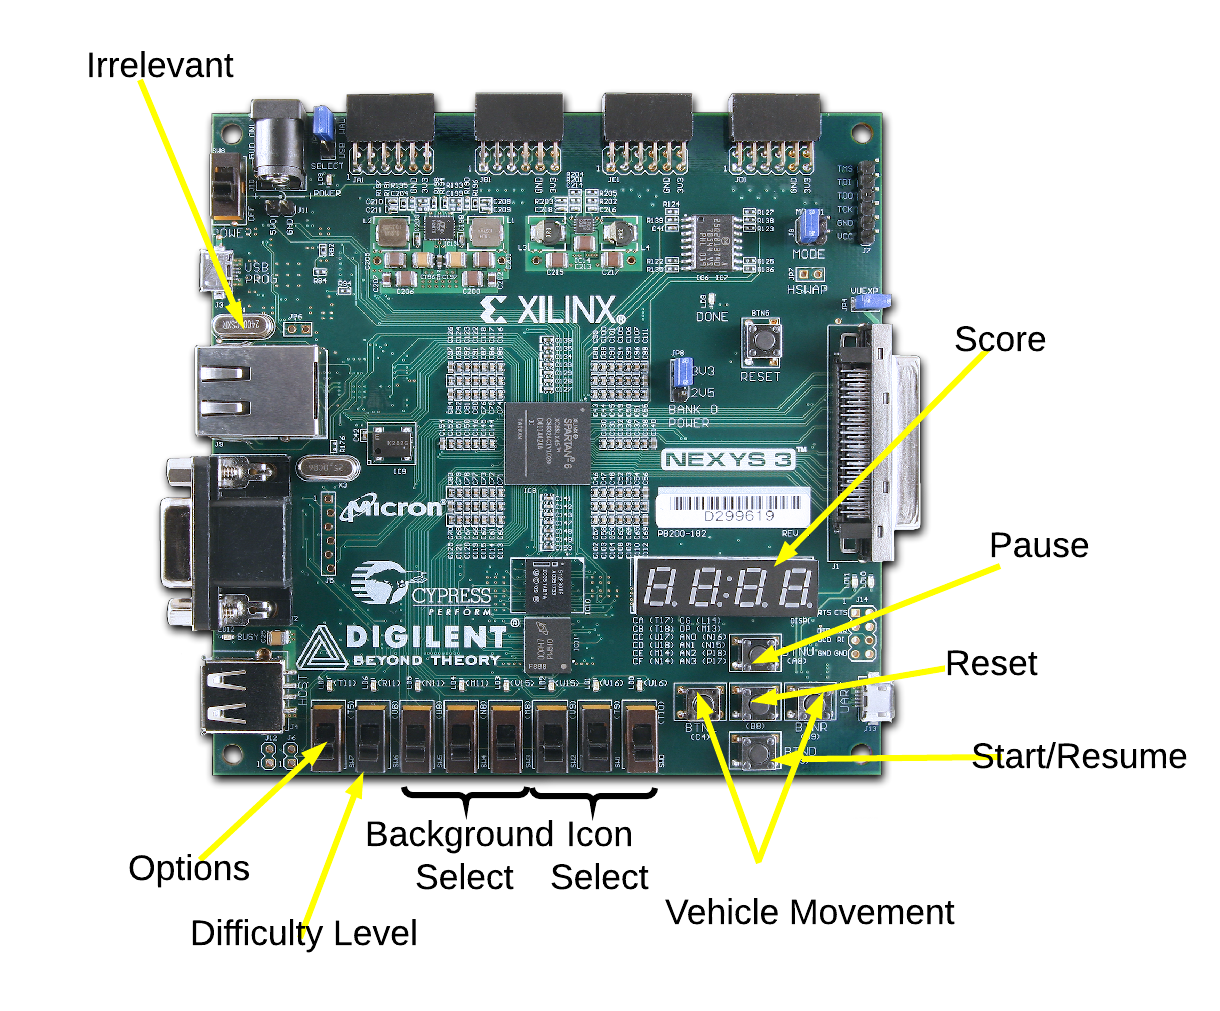
\includegraphics[height=0.8\textwidth, width=0.8\textheight]{Images/controls_mockup.png}
		\caption{Player Controls}
			\label{controls}
		\end{figure}	
	 	

\subsection{Features}
\textbf{Tunnel Vision} features both starting and ending screens. The courses are generated randomly through a pseudo-random number generator. Additionally, the LEDs are lit with certain patterns depending on the action the player is taking. If the player selects the harder difficulty, the score is incremented at a faster rate and with a multiplier, awarding them a higher score for the same distance travelled.	

\section{Implementation}

	\begin{figure}[h]\centering
	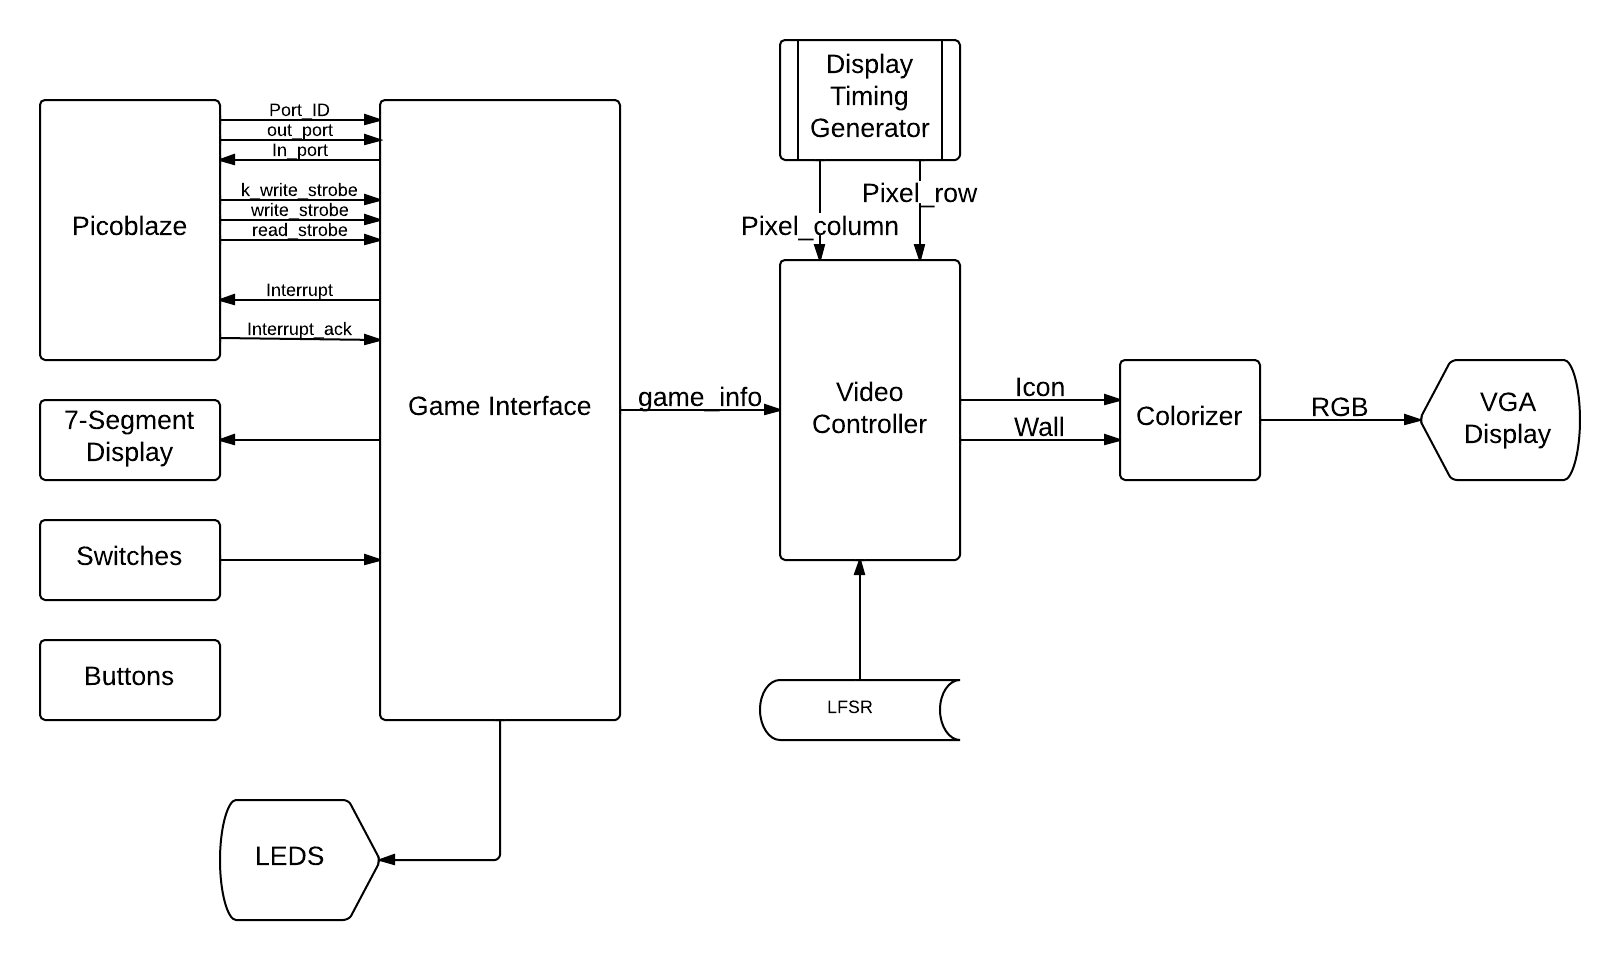
\includegraphics[height=0.7\textwidth, width=0.7\textheight]{Images/gameplay_diagram.png}
	\caption{Game Play Block Diagram}
		\label{block_diagram}
	\end{figure}	
		
The information controlled in the \textbf{PicoBlaze} core is sent to the \texttt{Video\_controller} module via the \texttt{game\_interface} module.  This information is constructed in an 8-bit register called \texttt{game\_info}.  The allocation of bits is seen in Figure \ref{game_info_bits}.  Collisions, obstacles, and icon changes were controlled in hardware.  The video controller receives the inputs of game\_info register and the \texttt{LFSR} module, shifted the wall appropriately, and used the collision logic to stop the game and display the \textbf{Game Over} screen.

\subsection{Software}

					
		\begin{figure}[h]\centering
		  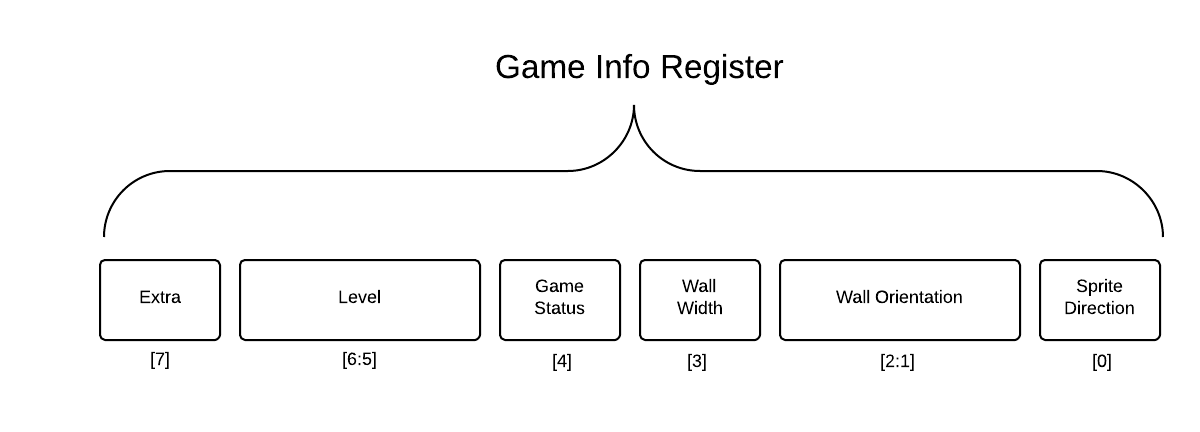
\includegraphics[width=.6\textwidth]{Images/game_info_bits.png}
		  \caption{Allocation of bits in game\_info register}
		  \label{game_info_bits}
		\end{figure}	

		\begin{figure}[h!]\centering
		  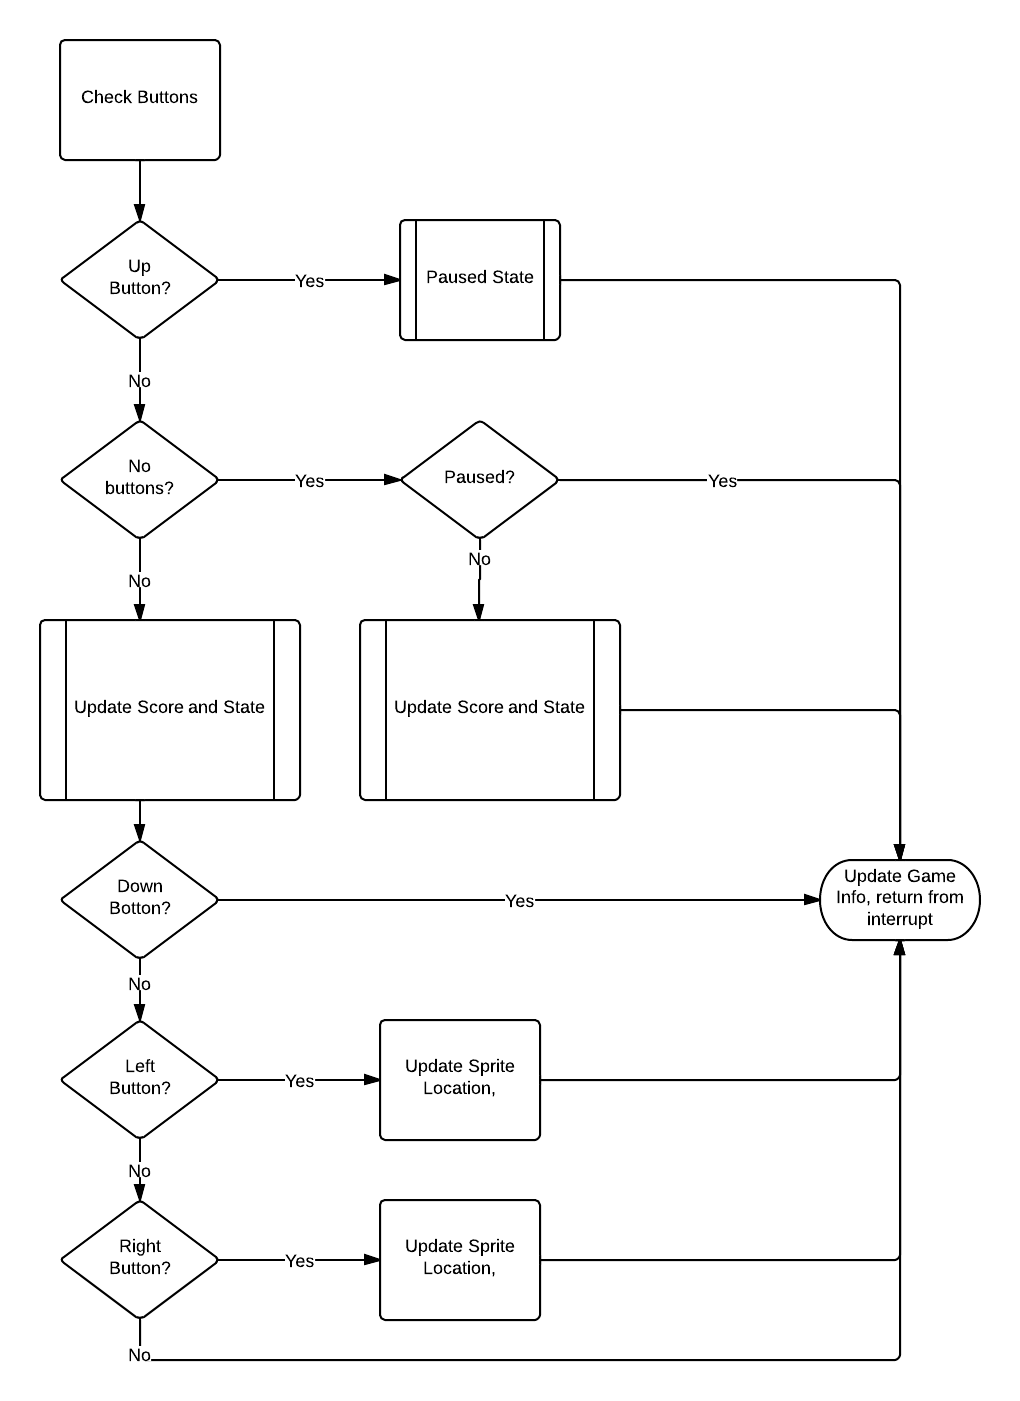
\includegraphics[width=.8\textwidth]{Images/game_logic.png}
		  \caption{Flowchart of Picoblaze Logic}
		  \label{game_logic}
		\end{figure}	


In order to ensure the correct flow of game play, the push button inputs were checked in the order seen in Figure \ref{game_logic}.  Each button check performs approximately the same function.  The push button input is checked, all other bits not pertaining to the specific button are masked off, and the button value is checked.  If it has not been pressed, the next button check is called.  If it has been pressed, the state is updated accordingly and the LEDs output the desired pattern. 
\vspace{12pt}
\begin{lstlisting}[caption=Function checking if the top button has been pushed, label=chk_up_btn]		
		FETCH		s2,		SP_BTN						;load saved debounced button
		AND			s2,		MSK_BTN_UP				;mask with up button
		COMPARE	s2,		MSK_BTN_UP
		JUMP 		NZ, 	chk_no_btn				;go to next phase if no up button
		LOAD 		s3,		PAUSED_STATE			;else pause and send out that register
		STORE		s3,		STATE
		FETCH		s3,		SP_GAME_INFO
		LOAD 		s4,		GAME_PAUSED 			;update game_info paused	
		AND			s3,		s4						
		STORE		s3,		SP_GAME_INFO
		LOAD		s5,		FF								;output LED pattern
		OUTPUT	s5,		PA_LEDS
		RETURN	
 \end{lstlisting}
\vspace{12pt}
\hspace{16pt}If the game is active and another button than the top one has been pressed, the \texttt{active} function is called.  This updates the state, score, and \texttt{game\_info} output.  In addition, when the left or right button has been pressed, the location of the vehicle is appropriately.\\

\vspace{12pt}
%include active function

\begin{lstlisting}[caption=Update the state and game info, label=active]		
		CALL				update_score				
		LOAD 	s3,		ACTIVE_STATE
		STORE	s3,		STATE
		FETCH	s3,		SP_GAME_INFO
		LOAD 	s4,		GAME_ACTIVE
		OR		s3,		s4					
		STORE	s3,		SP_GAME_INFO
		RETURN
 \end{lstlisting}


\hspace{16pt}In order to show the score over 4 digits, the \texttt{update\_score} function increments the least significant digit until 10 is reached.  At this point, the next significant digit counter is called and the previous value cleared.  This algorithm continues throughout all four digits. A separate function, \texttt{display\_score}, was created to actually load the stored score values to be displayed.  This structure was chosen to allow for the score to still update even if the 7-segment display is used for another output.  Future modifications to the game may make use of this function.\\		

\hspace{16pt} The difficulty level of \textbf{Tunnel Vision} can be changed by toggling switch 4 (Figure \ref{controls}). When the user has switched levels, the speed of the game increases.  This information is also sent in the game\_info register (Figure \ref{game_info_bits}).  The speed control is doubled, but the score increases at a 5:4 proportion.  This scaling is accomplished by modifying the counter in the \texttt{game\_interface} module that controls the speed of the interrupts. The speed is modified in the hardware portion.\\

	
\section{Video Controller Implementation}
	The video controller module, implemented in hardware, managed the icon switching and generation, the width and location of the walls, the obstacle creation, and the collision detection.
	
	%TODO finish this section up
	


\subsection{Walls}
The tunnel walls consist two red lines separated by a predefined width.  The walls directions are generated randomly using a linear feedback shift register. The video controller takes 2 bits from the LFSR and moves the walls left, right, or keeps them at the same position.  Since there are 4 possible numbers, the last possibility defaulted to keeping the walls at the same position.  \\

	\begin{figure}[h]\centering
	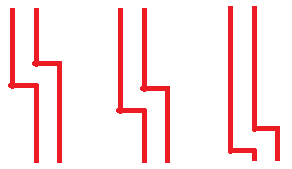
\includegraphics[height=0.3\textwidth]{Images/wall.png}
	\caption{Wall Location Transitions}
		\label{wall}
	\end{figure}

\hspace{12pt} The tunnel width, which is a function of time, decreases continuously as the user is playing the game. 
It is controlled by a flag that is set whenever the counter reaches a specific number. The wall speed is also monitored by a counter, which decides when to alter the wall location.  Figure \ref{wall} shows the transitions the wall would make based off one random value. \\

\hspace{12pt} Edge detection was performed in order to ensure the walls did not move out of bounds.  The coordinates of each side of the wall are checked, and if they are on the edge, the wall simply changes its next location to be closer to the middle.  \\
	
\subsection{Icons}

		\begin{figure}[h]\centering
		  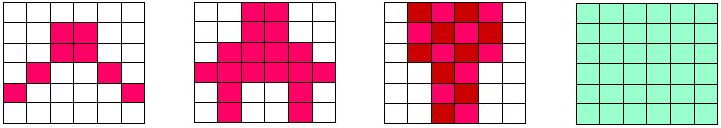
\includegraphics[width=.7\textwidth]{Images/icons.png}
		  \caption{Icons the user can select}
		  \label{icons}
		\end{figure}	

		There are currently four icons which can be selected by different switches on the board. The icons, just like the obstacles, background images, and walls, were created by directly coding the images into bits (Listing \ref{hammer}) instead of reading the image from a \texttt{coe} file. When the \texttt{pixel\_row} and \texttt{pixel\_column} signals reach the location of the icon, they are displayed on the screen. At all other times the icon acts transparent. The icons are ``animated'' by interchanging different colored icons of the same shape. The hammer in Figure \ref{icons} is an example of this.  \\
\hspace{12pt} The vehicle's location is updated based on the \texttt{game\_control} register coming from the Picoblaze soft core. Whenever the display timing generator has finished displaying a full screen and its coordinates are back at the origin, a counter is checked to decide whether the vehicle's location should change, regardless of the push button inputs.  Only when this counter is zero will the location be updated.  This effectively allows us to control the ``sensitivity'' of the vehicle by modifying the counter value. 

\begin{lstlisting}[caption=Example Icon creation (hammer), label=hammer]		
			if(i == 1 && (j==0 || j==1 || j==2))
				bitmap_bot_4[i][j] = 2'b11;			
			else if(i == 2 )
				bitmap_bot_4[i][j] = 2'b11;	
			else if(i ==3)
				bitmap_bot_4[i][j] = 2'b11;			
			else if(i == 4 && (j==0 || j==1 || j==2))
				bitmap_bot_4[i][j] = 2'b11;						
			else
				bitmap_bot_4[i][j] = 2'b00;	
 \end{lstlisting}



\subsection{Collision Detection}	
		Collisions are detected by comparing the coordinates of the wall or obstacle with the coordinates of the icon.  If they are equivalent, the collision detect is asserted, which is checked every clock edge. Once this occurs, the game stops and a ``Game Over'' screen is displayed.  

\begin{lstlisting}[caption=Collision Detection Logic, label=collision]		
	if ((Pixel_row >= locY) && (Pixel_row <= (locY + 3'h6)) && (Pixel_column >= locX) && (Pixel_column <= (locX + 4'h6)) ) begin
		collison_detect <= 1'd1;
	end	
 \end{lstlisting}
 
 
\subsection{Obstacles}
	Obstacles randomly appear on either side in the tunnel and also employ collision detection.  They take the icon's size (6x6) and extend the height to transform into a rectangular shape. The direction of the wall is also based on the LFSR, and is constrained to either be on the left or right side of the tunnel.
		
\subsection{Colorizer}

The \texttt{colorizer} module displays the icon and tunnel walls pixel by pixel.  Table \ref{colorizer} summarizes the color scheme used for wall and icon.
 
	\begin {table}
	\begin {center} 
	\vspace{15pt}
	
	\begin{tabular}{||c|c|c|c||}\hline	
		\textbf{Wall}	&	\textbf{Icon}	&	\textbf{Color}	&	\textbf{Purpose}		\\\hline
		00		&	00		&	White 	&	Background 	\\\hline
		01		&	00		&	Green 	&	Background (Trees) 		\\\hline
		10		&	00		&	Red 	&	Obstacles \& Walls 	\\\hline
		11		&	00		&	Gray 	&	Background	\\\hline
		X		&	01		&	Maroon	&	Icons		\\\hline
		X		&	10		&	Cyan	&	Icons \& Splash Screens	\\\hline
		X		&	11		&	Magenta	&	Icons \& Splash Screens	\\\hline	
	\end{tabular}
		\caption {Color Schemes} \label{colorizer}
	\end{center}
	\end{table} 		


%		\end{minipage}
%		\end{figure}
%
%		\begin{figure}[t!]\centering
%		\includegraphics[height=0.3\textwidth]{colorizer_table.png}
%		\caption{Colorizer Table}
%			\label{colorizer_table}
%		\end{figure}


%		\begin{figure}
%		\centering
%		\begin{minipage}{.5\textwidth}
%		  \centering
%		  \includegraphics[width=.6\textwidth]{icon_bitmap_3.png}
%		  \caption{Regular Image Translation}
%		  \label{reg_translation}
%		\end{minipage}%
%		\begin{minipage}{.5\textwidth}
%		  \centering
%		  \includegraphics[width=.6\textwidth]{icon_bitmap_4.png}
%		  \caption{Tilted Image Translation}
%		  \label{tilted_translation}
%		\end{minipage}
%		\end{figure}

		
		
		% first column
%\begin{minipage}[l]{0.5\textwidth}
%		\begin{itemize}

		
%\end{itemize}
%\end{minipage}\begin{minipage}[r]{0.5\textwidth}
%	\hspace{20pt}\includegraphics[width=0.9\textwidth]{../resources/mockup.png}
	
%	\hspace{50pt}Figure 1: Mockup of game screen


\section{Conclusion}


	\subsection{Challenges}
		
		\begin{itemize}				
		
		\item \textbf{Debugging}. Finding errors in our code proved to be difficult due to the length of time synthesis takes. We were forced to view the output on the screen to resolved issues, which was not very practical.  Debugging assembly language was also quite tedious, as there aren't any helpful warning or error messages.
%		\item \textbf{ROM for map that dynamically changes}. We attempted to add memory in order to change the collision detection and dynamically switch wall coordinates, but this was not able to be implemented.
		
		\item \textbf{Integration between hard-coded images and script generated images}.  We had trouble getting the different icons and splash screens created with Perl script to work with our current icon implementation.  Ultimately, these graphics are only used in the report and final presentation.
				
		\end{itemize}

	%table "Division of Tasks" 
	\begin {table}[H]
	\begin {center} 
	
	\begin{tabular}{||l|c|c|c|c||}\hline	
										& Erik  	& Bhavana  & Rohan  	& Nikhil\\\hline
	Game Logic				 			&	\checkmark 	&					&				 	&			\\\hline
	Video Controller					&	\checkmark	&	\checkmark		&	\checkmark		&			\\\hline
	Icons and Walls						&				&	\checkmark		&					&			\\\hline	
	Graphics							&				&	\checkmark		&	\checkmark			&	\checkmark		\\\hline
	Random Number Generation			&				&					&	\checkmark		&			\\\hline
	Documentation, Source Control		& 	\checkmark	&					&					& \\\hline
	
	\end{tabular}
		\caption {Division of Tasks} \label{Division of Tasks}
	\end{center}
	\end{table}
	\subsection{Future Work}
	
	\begin{itemize}
	\item \textbf{ROM Map:} The current implementation of wall generation does not use any memory.  If this functionality was converted to be stored in a ROM, different wall widths could be displayed in one frame, and collision detection could be done based off of the coordinates themselves. 
	\item \textbf{Improved Graphics:} Creating more icons and backgrounds would improve the game's aesthetic appeal.
	\item \textbf{Powerups and Bonuses:} Certain objects could give the player an extra life or a slower game speed.
	\item \textbf{Multiplayer Mode:} Two different tunnels could be generated, allowing multiple players to compete against each other. 
	
	\end{itemize}

Creating \textbf{Tunnel Vision} was an enjoyable experience (for the most part).  While we did face some roadblocks, we were pleased with the overall result.  There are many different paths we can take in the future to add new features to this game.	

		\begin{figure}[h]\centering
		  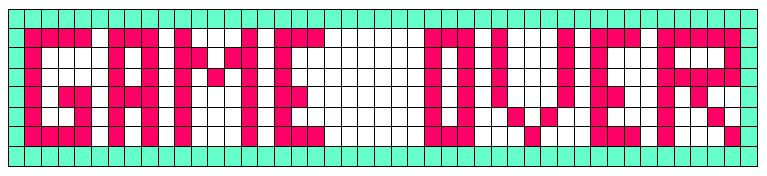
\includegraphics[width=.8\textwidth]{Images/gameover_screen.png}
		  \label{gameover_screen}
		\end{figure}		
	
%\vspace{-20pt}
%		\begin{figure}[h]
%		  \begin{flushright}
%		  
\includegraphics[width=.1\textwidth]{Images/qrcode.png}
%		  \label{qrcode}
%		  \end{flushright}
%		\end{figure}		
	
\end{document}